\documentclass[../../main.tex]{subfiles}

\begin{document}
In both designs described above, \texttt{MasterSecret} is returned to
the untrusted component. As previously mentioned, the
\texttt{MasterSecret} is used to compute the session key block; hence,
an adversary, after exploiting the untrusted component, may leak the
session key block, or leak \texttt{MasterSecret} and derive the
session key block themselves. Consequentially, an attacker may choose
to store session key blocks and eavesdropped sessions, and decrypt the
stored sessions at his leisure. Yet, requests received from the client
have to be in plain-text for processing by unprivileged user programs.
This section describes an augmentation to the designs presented above,
which attempts to resolve the highlighted issue, and explains the
resulting security properties.

A possible solution to the outlined problem would be to implement the
user programs that require plain-text as part of the \textit{enclave
  program} and, by extension, the TCB. As a result, session keys may
reside within the enclave, and, aside from packets that are plain-text
in the SSL/TLS handshake, all output from the \textit{enclave program}
to the unpriveleged/untrusted network facing component would be
encrypted. This design, however, introduces a large TCB that
incorporates all of the user-written code, making it difficult to
reason about its security.

Alternatively, we expanded upon the designs explained earlier as
follows: instead of returning the \texttt{MasterSecret} to the
untrusted component, we compute the session key block, and store it
within the enclave. We then provide a interface that allows the
untrusted component to decrypt data received from a client and an
interface to encrypt data outgoing to a client. These interfaces also
calculates the MAC using the \texttt{mac\_secret} from the session key
block (See Section~\ref{sec:ssloverview}).
Figure~\ref{fig:keys-inside} illustrates this design.

\begin{figure}[H]
  \centering
  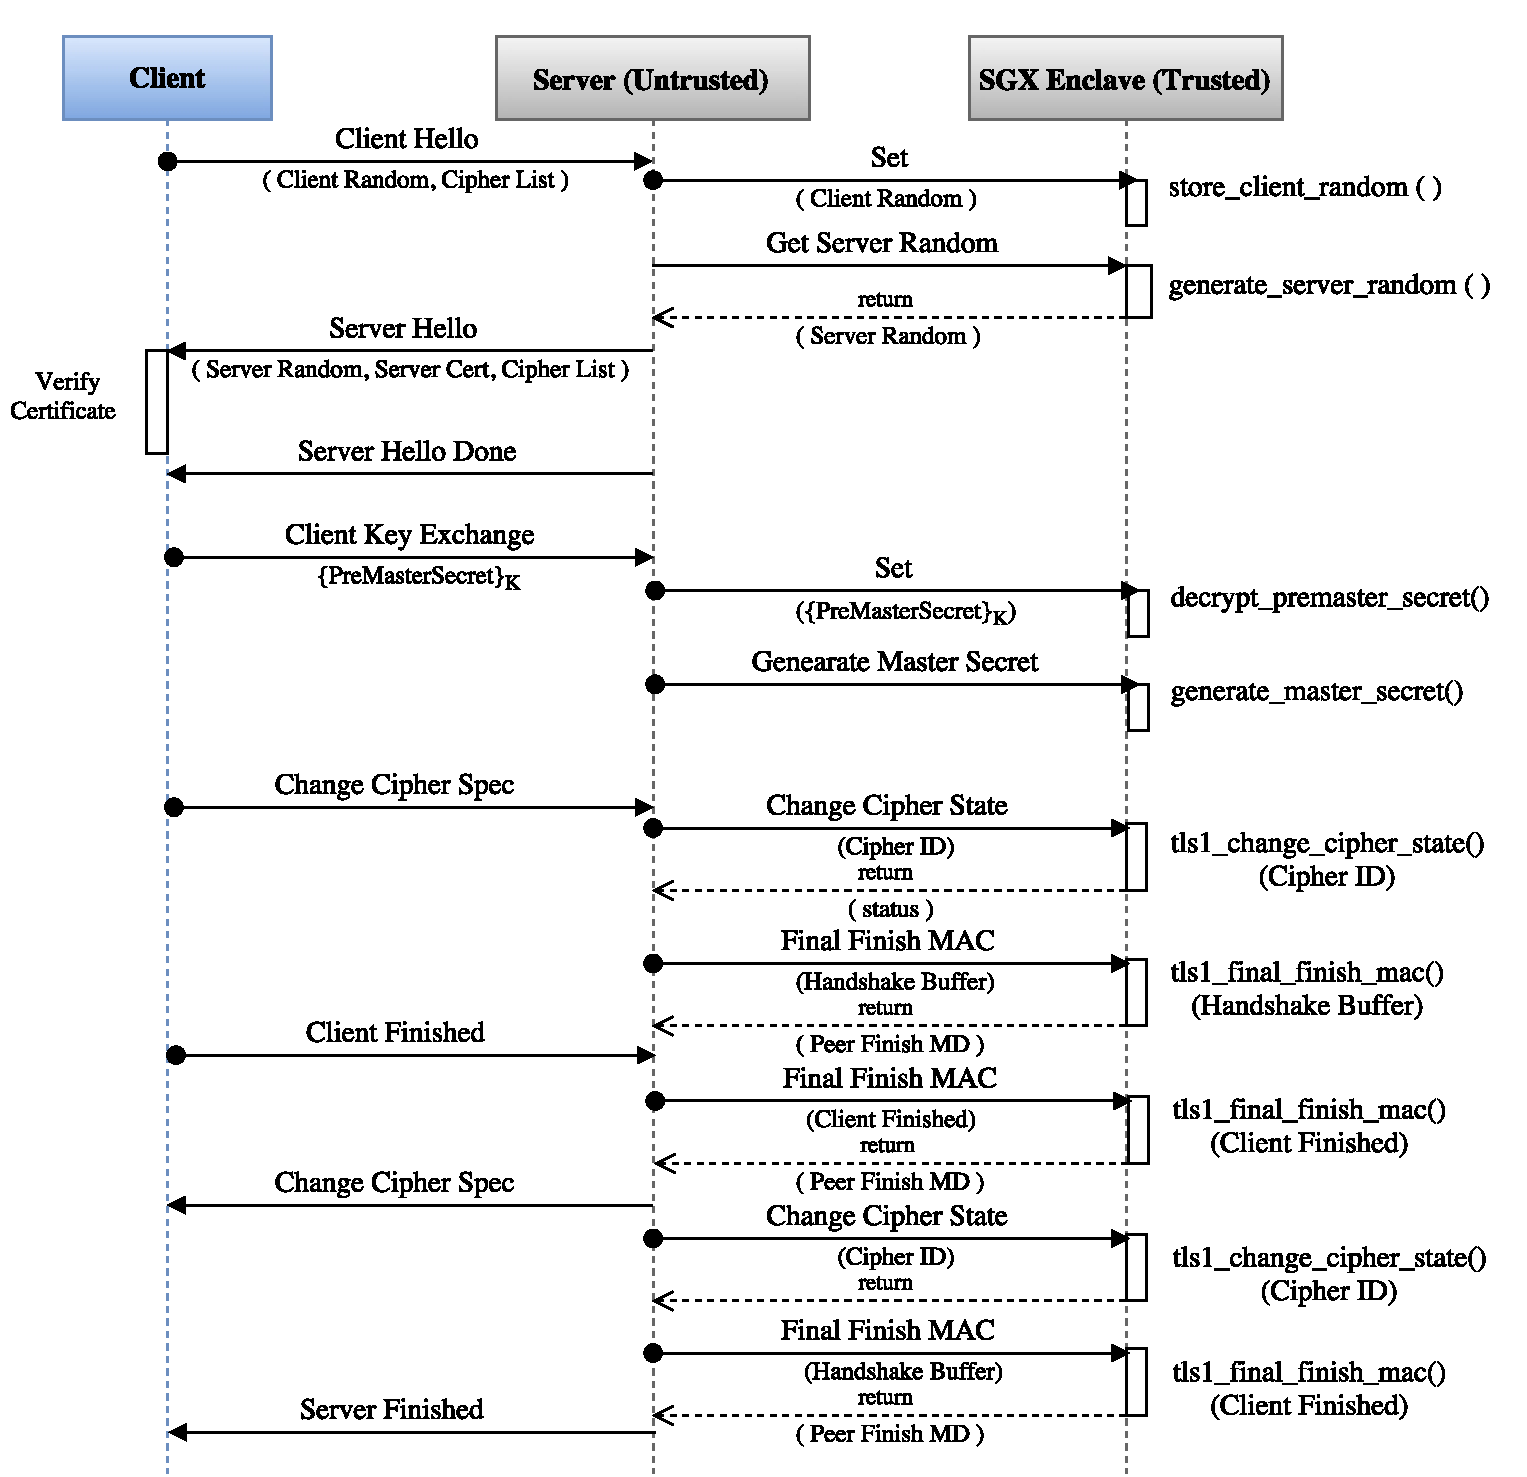
\includegraphics[scale=0.4]{images/RSA-SGX-Handshake-SessionKeys.pdf}
  \caption{SSL/TLS handshake with session keys in the enclave}
  \label{fig:keys-inside}
\end{figure}

As before, the untrusted component obtains \srandom~from the
\textit{enclave program}. The untrusted component then forwards
packets received to allow for the generation of
\texttt{PremasterSecret}. Its at this step that new design elements
appear. First, \texttt{MasterSecret} is no longer returned to the
untrusted component. Second, the \texttt{Change\-CipherSpec} message
is passed to the client. This is because \texttt{ChangeCipherSpec}
indicates to the recepient the transition to using the just-negotiated
keys; therefore, the message is forwarded to the \texttt{enclave
  program} to signal the need for generating the session key block,
and initializng a cipher specific
context\footnote{\texttt{ChangeCipherSpec} signals the transition to
  the symmetric cipher, indicating that all packets exchanged beyond
  this point are encrypted in the just-negotiated keys. The most
  commonly used symmetric cipher in SSL/TLS is AES.}. Next, the server
prepares for receiving the \texttt{ClientFinished} message by
beginning the calculation of a cryptographic digest\footnote{This is
  more of an implementation consideration, than a design issue. The
  RFC for TLS 1.2 does not specify the instance of time at which the
  calculation of the \texttt{FinalFinish MAC} completes, only its
  components. However, this multi-step approach is common across
  popular SSL/TLS libraries, and we, therefore, elected to support
  it.} of the handshake messages received so far (handshake digest)
\footnote{As defined by the RFC for TLS 1.2, the digest enclosed in a
  participant's \texttt{Finished} message does not include the other
  side's \texttt{Finished} message.} required for the
\texttt{ServerFinished} message. This message contains the
\texttt{FinalFinish MAC}, a PRF that takes an input of
\texttt{MasterSecret} and the handshake digest. Since
\texttt{MasterSecret} is no longer returned to the untrusted
component, this PRF must be calculated in the \textit{enclave
  program}. Moreover, the \texttt{ServerFinished} message is
encrypted; the \textit{enclave program} encrypts it before returning
it to the untrusted component. Finally, upon receiving the encrypted
\texttt{ClientFinished} message, the untrusted component forwards the
message to the \textit{enclave program} for decryption and
verification. This is carried out by invoking the decrypt interface
which also calculates the MAC of the decrypted message to verify its
authenticity and integrity. If this process is completed successfully,
the server may now send the \texttt{ChangeCipherSpec} message to the
client, signalling the transition to the symmetric cipher and sets up
the appropriate cipher environment in the enclave as well. Finally,
the untrusted component signals the \texttt{enclave program} to
complete the computation of the \texttt{FinalFinish MAC}, forwarding
the remainder of the handshake buffer. The server now sends the
\texttt{ServerFinished} message, completing the connection
establishment step. If the client successfully verifies the
\texttt{ServerFinished} message, the SSL/TLS connection is considered
established. Note that, as the protocol defines, the interface used
for encryption/ decryption of the \texttt{Finished} messages is the
same used for encryption/ decryption of the user data travelling over
the network. Thus, every subsequent data record will be
encrypted/decrypted by the same interface used for
encrypting/decrypting the \texttt{Finished} messages, with the session
keys never being exposed to the untrusted component
\footnote{Figure~\ref{fig:keys-inside} shows an additional invocation
  of \texttt{Change\-Cipher\-State} which we did not explain. SSL/TLS
  libraries implement encryption and decryption for symmetric ciphers
  in one function. To allow for such an implementation, there is a
  second function that changes the state of the encrypt/decrypt
  function. We included this invocation in the Figure for
  completeness, however, it is an implementation detail.}.

While this design exposes a decrypt/encrypt interface, providing an
\textit{oracle} for the session keys, it remains more secure than a
design where the session keys remain in the untrusted componenet. Even
though an adversary may exploit the untrusted componenet and
encrypt/decrypt packets of their choosing, there are a few
limitations:
\begin{itemize}
  \item Packets that are encrypted or decrypted can only pertain to
    a currently ongoing session. This is because, after a session
    terminates, the session keys are removed from the enclave, and, thus,
    invoking the interface with packets from previously eavesdropped
    sessions does not return any useful results (this relies on the
    freshness property, discussed earlier, ensuring that new session keys
    are generated for each session in a manner that cannot be influenced
    by the adversary).
  \item Under this scheme, an adversary cannot leak the session keys
    by exploiting the untrusted component. Consequintially, to acquire
    any useful data through encrypting/decrypting packets, the adversary
    must remain connected to the server machine, actively exploiting it.
    This is much more difficult to concealthan the attack described
    at the beginning of this subsection where the attacker leaks the session
    keys and decrypts/encrypts packets on another machine.
\end{itemize}
These security benefits, nevertheless, come at a performance overhead
that we discuss in Section~\ref{sec:perfeval}.


\end{document}

%%% Local Variables:
%%% mode: latex
%%% TeX-master: "../../main"
%%% End: